% Tamaño de letra.
\documentclass[12pt,titlepage]{article}

%------------------------------ Paquetes ----------------------------------

% Paquetes:

%Para comentarios multilínea.
\usepackage{verbatim}

% Para tener cabecera y pie de página con un estilo personalizado.
\usepackage{fancyhdr}

% Codificación UTF-8
\usepackage[utf8]{inputenc}

% Castellano.
\usepackage[spanish]{babel}

% Tamaño de página y márgenes.
\usepackage[a4paper,headheight=16pt,scale={0.75,0.8},hoffset=0.5cm]{geometry}

% Para poder agregar notas al pie en tablas:
%\usepackage{threeparttable}

% Tipo de letra Helvetica (Arial).
%\usepackage{helvet}
%\renewcommand\familydefault{\sfdefault}

% Gráficos:

% Para incluir imágenes, el siguiente código carga el paquete graphicx
% según se esté generando un archivo dvi o un pdf (con pdflatex).

% Para generar dv.
%\usepackage[dvips]{graphicx}

% Para generar pdf.
\usepackage[pdftex]{graphicx}
\pdfcompresslevel=9
\usepackage{appendix}
\usepackage{pdfpages}

\usepackage{url}


%
% Directorio donde están las imagenes.
%
%\newcommand{\imgdir}{includes}
%\graphicspath{{\imgdir/}}

%------------------------------ ~paquetes ---------------------------------

%------------------------- Inicio del documento ---------------------------

\begin{document}

% ---------------------- Encabezado y pie de página -----------------------

% Encabezado: sección a la derecha.
% Pie de página: número de página a la derecha.

\pagestyle{fancy}
\renewcommand{\sectionmark}[1]{\markboth{}{\thesection\ \ #1}}
\lhead{}
\chead{}
\rhead{\rightmark}
\lfoot{}
\cfoot{}
\rfoot{\thepage}

% ---------------------- ~Encabezado y pie de página ----------------------

% -------------------------- Título y autor(es) ---------------------------

\title{ConcuShare}
\author{}

% -------------------------- ~Título y autor(es) --------------------------

% ------------------------------- Carátula --------------------------------

\begin{titlepage}

\thispagestyle{empty}

% Logo facultad más pie de la figura.
\begin{center}

\includegraphics[scale=0.55]{./Images/fiuba}\\
\large{\textsc{Universidad de Buenos Aires}}\\
\large{\textsc{Facultad De Ingeniería}}\\
\small{Año 2012 - 2\textsuperscript{do} Cuatrimestre}
\end{center}

\vfill

% Título central.
\begin{center}

\Large{\underline{\textsc{Sistema de Programaci\'on No Convencional de Robots}}}
\Large{\underline{\textsc{(75.70)}}}

\vfill

% Tabla de integrantes.

\Large{\underline{\textsc{Trabajo Pr\'actico}}}

\vfill

\Large\underline{Integrantes} \linebreak\linebreak

% Separación entre columnas.
\large\addtolength{\tabcolsep}{-3pt}
% Tres columnas con alineación centrada.
\begin{tabular}{|| c | c | c ||}
\hline
\textbf{Apellido, Nombre} & \textbf{Nro. Padrón} & \textbf{E-mail} \\
\hline
Bukaczewski, Verónica & 86954 & vero13@gmail.com \\
\hline
Rivero, Hern\'an & XXXXXX & riverohernanj@gmail.com \\
\hline
\end{tabular}
\end{center}

\vfill

\hrule
\vspace{0.2cm}

% Pie de página de la carátula.
%\noindent\small{75.70 - Sistema de Programaci\'on No Convencional de Robots \hfill}

\end{titlepage}

% ------------------------------- ~Carátula -------------------------------

% ----------------------- Cabeceras y pies de página ----------------------

\pagestyle{fancy}
\lhead{}
\chead{}
\rhead{}
\lfoot{\scriptsize{75.70 - Sistema de Programaci\'on No Convencional de Robots \\
\\Trabajo práctico 0 - 2do cuatrimestre 2012}}
\cfoot{}
\rfoot{\\\thepage}
\renewcommand{\headrulewidth}{0pt}

% ---------------------- ~Cabeceras y pies de página ----------------------

% -------------------------------- Índice ---------------------------------

% Hago que las páginas se comiencen a contar a partir de aquí.
\setcounter{page}{2}

% Índice.
\newpage
\thispagestyle{empty}
\tableofcontents
\newpage

% -------------------------------- ~Índice --------------------------------

% ----------------------------- Inicio del tp -----------------------------

\section{Objetivo}
El objetivo del presente trabajo pr\'actico es familiarizarnos con la herramienta Joone, utilizada para el estudio de Redes Neuronales. Y finalmente, poder realizar una an\'alisis de los resultados obtenidos.

\section{Descripci\'on base de datos seleccionada}
Se seleccion\'o la base de datos del TA-TE-TI, extra\'ida de la p\'agina UCI (Machine Learning Repository) \cite{UCI}. Esta base de datos codifica el conjunto completo de configuraciones posibles para el final del juegos del TA-TE-TI, donde "x" se supone que juega primero. El concepto objetivo es "ganar para x" (es decir, ocurre cuando "x" tiene una de las 8 posibles maneras de crear un "tres-en-l\'inea").

\subsection{Informaci\'on relevante}

\begin{itemize}
 \item N\'umero de instancias: 958.
 \item N\'umero de atributos: 10.
 \item Informaci\'on de los atributos: (x=player x has taken, o=player o has taken, b=blank)
    \begin{enumerate}
      \item top-left-square: {x,o,b}
      \item top-middle-square: {x,o,b}
      \item top-right-square: {x,o,b}
      \item middle-left-square: {x,o,b}
      \item middle-middle-square: {x,o,b}
      \item middle-right-square: {x,o,b}
      \item bottom-left-square: {x,o,b}
      \item bottom-middle-square: {x,o,b}
      \item bottom-right-square: {x,o,b}
      \item Class: {positive,negative}
    \end{enumerate}
 \item Falta de valores de atributo: Ninguno.
 \item Distribución de Clase: 65,3\% son positivos (es decir, gana para "x").
\end{itemize}

\section{Preparando los datos para las corridas}
Los valores para los atributos fueron modificados para que el programa Joone pueda ejecutarse correctamente;
debido a que s\'olo trabaja con n\'umeros reales y enteros. \\
{\bf{Valores:}}
    \begin{enumerate}
      \item x= +1
      \item o= -1
      \item b= 0
      \item positive= 1
      \item negative= 0
    \end{enumerate}

\section{Red Neuronal}

\begin{center}
 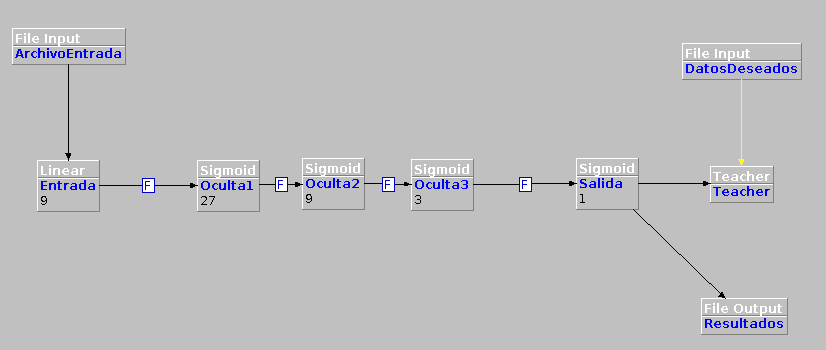
\includegraphics[width=500,height=250]{./Images/RN.png}
 % RN.png: 826x350 pixel, 96dpi, 21.85x9.26 cm, bb=0 0 619 262
\end{center}

\section{Ejecutando la Red Neuronal}
\begin{center}
 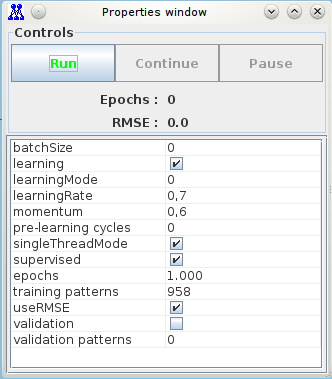
\includegraphics{./Images/configuracion-corridas.png}
 % configuracion-corridas.png: 333x368 pixel, 96dpi, 8.81x9.74 cm, bb=0 0 250 276
\end{center}

\begin{center}
 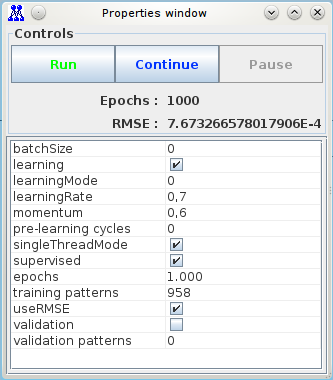
\includegraphics{./Images/fin-corridas.png}
 % fin-corridas.png: 332x366 pixel, 96dpi, 8.78x9.68 cm, bb=0 0 249 274
\end{center}

\section{Resultados}
Luego del aprendizaje que se le aplic\'o a la Red Neuronal, se agreg\'o un archivo de salida para probar la red entrenada (``Resultados.txt''). Para ello, se configur\'o: 
\begin{itemize}
 \item learning = FALSE
 \item epochs = 1
\end{itemize}
En el archivo se pudo observar que los valores coinciden apr\'oximadamente con la columna diez de la base de datos original. 

\section{Conclusiones}
Cuanto lleva armarlo y cuando lleva correrlo. \\


% -------------------------------- Apendice --------------------------------
\appendix
\newpage
\section{Tabla comparativa de los resultados}
A continuaci\'on se presentan los resultados originales de la base de datos contra los obtenidos de la red neuronal entrenada.

% ------------------------------- ~Apendice -------------------------------

% ----------------------------- Bibliografia ------------------------------
\newpage
\begin{thebibliography}{99}
	\bibitem{docjoone}
		\textbf{Documentaci\'on Joone} \\
		\url{http://sourceforge.net/projects/joone/files/Documentation/DTE/JooneDTEGuide.pdf}

	\bibitem{tutorialjoone}
		\textbf{Tutorial B\'asico Joone} \\
		\url{http://ubuntuone.com/p/1dB/}

	\bibitem{UCI}
		\textbf{UCI Machine Learning Repository - Tic-Tac-Toe Endgame Data Set} \\
		\url{http://archive.ics.uci.edu/ml/datasets/Tic-Tac-Toe+Endgame}

	\bibitem{tic-tac-toe1}
		\textbf{Training an artificial neuronal network to play tic-tac-toe} \\
		\url{http://users.auth.gr/kehagiat/GameTheory/12CombBiblio/TicTacToe.pdf}

	\bibitem{tic-tac-toe2}
		\textbf{How to code an artificial neural network (Tic-tac-toe)?} \\
		{\url{http://stackoverflow.com/questions/761216/how-to-code-an-artificial-neural-network-tic-tac-toe}}

	\bibitem{tic-tac-toe3}
		\textbf{Neural Net Training for Tic-Tac-Toe} \\
		\url{www.cs.virginia.edu/~bmb5v/cs660/Project.doc}

	\bibitem{tic-tac-toe4}
		\textbf{TD Learning of Game Evaluation Functions with Hierarchical Neural Architectures} \\
		\url{http://webber.physik.uni-freiburg.de/~hon/vorlss02/Literatur/reinforcement/GameEvaluationWithNeuronal.pdf}

\end{thebibliography}

% ---------------------------- ~Bibliografia ------------------------------

% ------------------------------ Fin del tp -------------------------------

\end{document}

%---------------------------- Fin del documento ---------------------------

